\documentclass[10pt,twocolumn,letterpaper]{article}

\usepackage{cvpr}
\usepackage{times}
\usepackage{epsfig}
\usepackage{graphicx}
\usepackage{amsmath}
\usepackage{amssymb}
\usepackage{CJK}
\usepackage[utf8]{inputenc}
\usepackage{listings}
\usepackage[hyphens]{url}
\usepackage{color}

\graphicspath{ {images/} }

\definecolor{dkgreen}{rgb}{0,0.6,0}
\definecolor{gray}{rgb}{0.5,0.5,0.5}
\definecolor{mauve}{rgb}{0.58,0,0.82}

\lstset{frame=tb,
  aboveskip=3mm,
  belowskip=3mm,
  showstringspaces=false,
  columns=flexible,
  basicstyle={\small\ttfamily},
  numbers=none,
  numberstyle=\tiny\color{gray},
  keywordstyle=\color{blue},
  commentstyle=\color{dkgreen},
  stringstyle=\color{mauve},
  breaklines=true,
  breakatwhitespace=true,
  tabsize=3
}
\DeclareMathOperator{\argmax}{\arg\!\max}


% Include other packages here, before hyperref.

% If you comment hyperref and then uncomment it, you should delete
% egpaper.aux before re-running latex.  (Or just hit 'q' on the first latex
% run, let it finish, and you should be clear).
\usepackage[breaklinks=true,bookmarks=false]{hyperref}

\cvprfinalcopy % *** Uncomment this line for the final submission

\def\cvprPaperID{****} % *** Enter the CVPR Paper ID here
\def\httilde{\mbox{\tt\raisebox{-.5ex}{\symbol{126}}}}

% Pages are numbered in submission mode, and unnumbered in camera-ready
%\ifcvprfinal\pagestyle{empty}\fi
\setcounter{page}{1}
\begin{document}
\begin{CJK}{UTF8}{gbsn}

%%%%%%%%% TITLE
\title{Project 2}

\author{
% For a paper whose authors are all at the same institution,
% omit the following lines up until the closing ``}''.
% Additional authors and addresses can be added with ``\and'',
% just like the second author.
% To save space, use either the email address or home page, not both
}

\maketitle
%\thispagestyle{empty}

%%%%%%%%% ABSTRACT
\begin{abstract}

The theory of Reinforcement Learning (RL) is proven to be a good candidate to train an agent to interact with a certain environment. Previous work usually requires that the environment model is clearly built, which is not practical in applications, where sensor input cannot express the environment well. We choose the paper "Human-level control through deep reinforcement learning"~\cite{mnih2015human}, where this problem is addressed. Experiments on Atari 2600 games show that the proposed Deep Reinforcement Learning method achieves human level control on 29 of the 49 games. The experiments we do according to this paper gives out similar results in the finished training epochs.

\end{abstract}
\section{Introduction}
Reinforcement learning is proposed to solve the problem that how an agent optimizes its behavior within a certain environment. Usually, we model this problem with the following variables and functions:
\begin{itemize}
    \item \textbf{State $s$} is used to represent the state of the environment. 
    \item \textbf{Action $a$} denotes the action the agents take.
    \item \textbf{Reward $r$} denotes the target the agents is to maximize in the experiment.
    \item \textbf{Policy $\pi(s)$} receives the current environment state $s$ as input and returns the action that the agent should take.
\end{itemize}
RL is to solve the policy $\pi$ given the environment and reward at each time step to maximize the final reward.

One of the algorithm to solve this problem is Q-learning, whose idea is also adopted in this paper. In Q-learning, we try to model the value of an action $a$ given the environment state $s$, which is a function $Q(s, a)$ and the policy $\pi$ adopts the action with the maximum value at each time step. In traditional Q-learning, this function is first initialized as a table for each $(s, a)$ pair. Each entry in the table is updated iteratively during training. 

For enumerable number of states, it is possible to use the above strategy. But for more complex situations like games or for human being, we can only get a high dimensional visual input as $s$. In these cases, it is impractical to enumerate all the possible states. This limits the the application domain of RL.

In this paper, a deep neural network is used to model the value function $Q(s, a)$. Recently, neural network, especially convolutional neural network (CNN) is showing great performance in image processing over traditional algorithms. Researches in neural science also show that the hierarchical structure of neural network is similar to what our brain uses to processes signal. The main challenge in using deep neural network in RL is the way to train the network. Directly using traditional RL framework leads to difficulties in training deep neural network for several reasons. First, there is high correlations in a sequence of observations. Second, update to Q affects the policy and thus affects data distribution. Third, there is correlation between the action value $Q$ and the target value $r+\gamma Q(s^\prime, a^\prime)$.

To address these problems, this paper adopts two ideas, which are also the main contributions:
\begin{itemize}
    \item An experience replay method is used to randomizes the data to reduce correlation between observations, hence reinforces the long term sight of the agent.
    \item An iterative update strategy is used to reduce the correlation between action value and target value.
\end{itemize}
The experimental result in the paper shows that the network can achieve human level control on 29 of 49 of the Atari 2600 games. We adopt the network structure and replay the experiment on two of the tasks, Breakout and Space Invaders, which gives out similar results on the already finished training epochs. While there is still difference between our result and that reported in the paper.


\section {Methods}

The main contribution of this paper is to solve the training problems when using deep neural networks as the Q function for RL. Two strategies are used in the training process: memory replay and iterative update of target Q function.

\subsection{Memory Replay}

In traditional Q learning, the optimization process of Q function is done through a process of interacting with the environment. This leads to high correlations between adjacent data used to update Q. The memory replay strategy stores a set of experience $(s_t, a_t, r_t, s_{t+1})$ as the memory, which denotes that with environment $s_t$ at time $t$, the agent took action $a_t$, gets a reward $r_{t}$ and transfers the environment to $s_{t+1}$. Each time to train the network, an experience is randomly selected from the memory to apply back propagation on the network.

Note that, to accelerate the speed of training, the experiences in memory are collected during training but not before training. This means the correlation of data is high at the beginning of training. But in the long run, the correlation will be small.

\subsection{Iterative Update of Target Function}

\begin{figure}
\begin{center}
   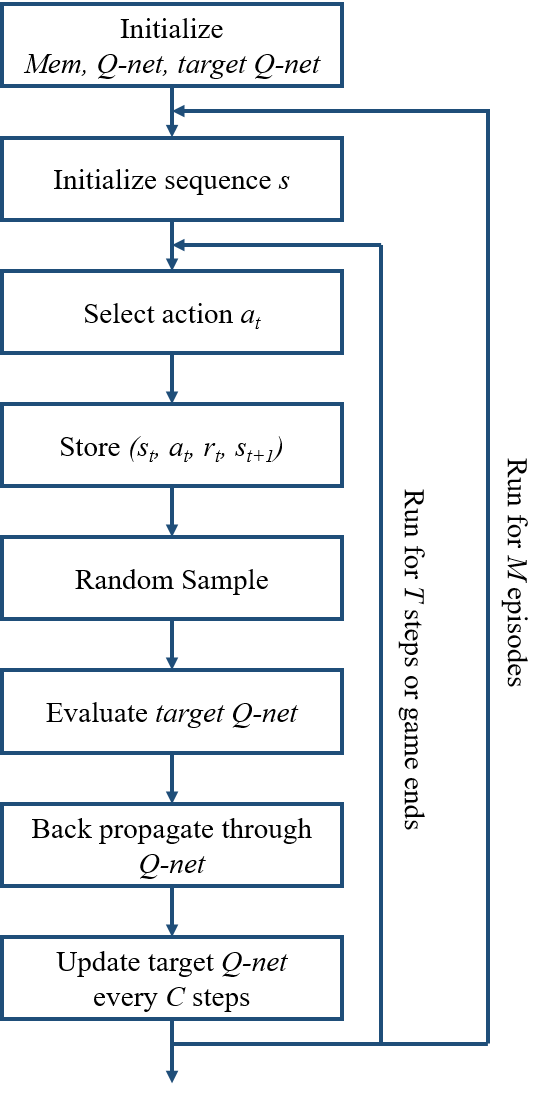
\includegraphics[width=0.9\linewidth]{flow.png}
\end{center}
\caption{Training flow graph}
\label{fig:flow}
\end{figure}

In general, the Q function measures the value of each action at a certain state $s$. The loss function can be expressed as:
\[
    L = r+\gamma \max\limits_{a^\prime} Q(s^\prime, a^\prime) - Q(s, a)
\]
If this loss is used to train $Q$ it self, there will be correlation between the target and the network output. In this paper, a separate network $\hat{Q}$ is used to calculate the target. During the training process, the network for $Q$ is updated each time. The parameters of $Q$ is copied to $\hat{Q}$ every $C$ cycles. In this way, $\hat{Q}$ converges to $Q$ if the training of $Q$ converges. But in each time of training, $\hat{Q}$ is different from $Q$ and thus the correlation between target and network output becomes lower.

\subsection{Training Flow}

The overall training flow proposed in this paper is shown in Figure~\ref{fig:flow}. $Q$ and $\hat{Q}$ network is randomly initialized first. In each training episode, a new game is started with state $s_0$. Within each cycle in an episode, first, an action $a_t$ is selected based on the function $Q$. This is done in an $\epsilon$-greedy policy to enable the agent to try other possible actions. Then $r_t$ and $s_{t+1}$ is got from the game and $(s_t, a_t, r_t, s_{t+1})$ is stored to the memory. Next, $s_{t+1}$ is used as the input to $\hat{Q}$ and the loss $L$ is got by:
\[
    L = r_t+\gamma \max\limits_{a_{t+1}} \hat{Q}(s_{t+1}, a_{t+1}) - Q(s_t, a_t)
\]
This loss is used to back propagate through $Q$ to update the weights of $Q$. Every $C$ cycles, the weights of $Q$ is copied to $Q^\prime$. An episode ends if the number of cycles reaches an upper bound or the game ends.



%%%%%%%%% BODY TEXT
\section{Implementation}

We use Tensorflow 0.12 \footnote{Tensorflow \url{https://www.tensorflow.org/}} and OpenAI Gym \footnote{OpenAI Gym \url{https://gym.openai.com/}} framework for our implementation. Tensorflow is an open source software library for numerical computation using data flow graphs, while OpenAI Gym is an open source interface to reinforcement learning tasks, including the Atari 2600 games.

\begin{figure}
\begin{center}
   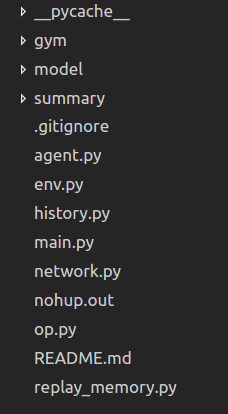
\includegraphics[width=0.9\linewidth]{code_architecture.png}
\end{center}
\caption{code architecture}
\label{fig:code_architecture}
\end{figure}

Figure \ref{fig:code_architecture} is the code architecture of our implementation. main.py contains the hyper parameters and some running options of our code. 

agent.py implements how to train the agent and how the agent play the Atari 2600 games using Deep Q-Network learning algorithm. It uses other modules. 

env.py module is a wrapper for the OpenAI Gym Atari 2600 game environment, and takes the preprocessing works described in the paper. 

history.py module implements the function $\phi$ that stack m most recent frames as input of the Q-function. 

network.py module implements the Q function, which is a CNN network. It uses some op from op.py module such as convolution op, liner op and clip error op, which can let the network more stable according to the paper. 

relay\_memory.py module implements the experience replay described in paper. The paper give a memory size of 1,000,000, which is really huge, consider of the complex structure of one memory cell. To make it more space efficiency so that can fits to our servers, we did some optimization. Original structure of memory cell is $(\phi_t, a_t, r_t, \phi_{t+1})$, in which $\phi$ is the m most recently frames $[s_{t-m+1}, s_{t-m+2}, ..., s_{t-1}, s_t]$. But we can only store $(a_t, r_t, s_{t+1})$ as a memory cell without the redundancy and restore the whole $(\phi_t, a_t, r_t, \phi_{t+1})$ from most recent frames we saved. In that way we lower the memory demand to $\frac{1}{2m}$ of original one.

Change the flag parameters in main.py and run 
\begin{lstlisting}
python main.py
\end{lstlisting}
will start training or playing. Run 
\begin{lstlisting}
tensorboard --logdir="./summary"
\end{lstlisting}
can see the interactivity graph in your browser.

\section{Experiments}

\subsection{Hyper Parameters and Tricks in Training}

\begin{figure}
\begin{center}
   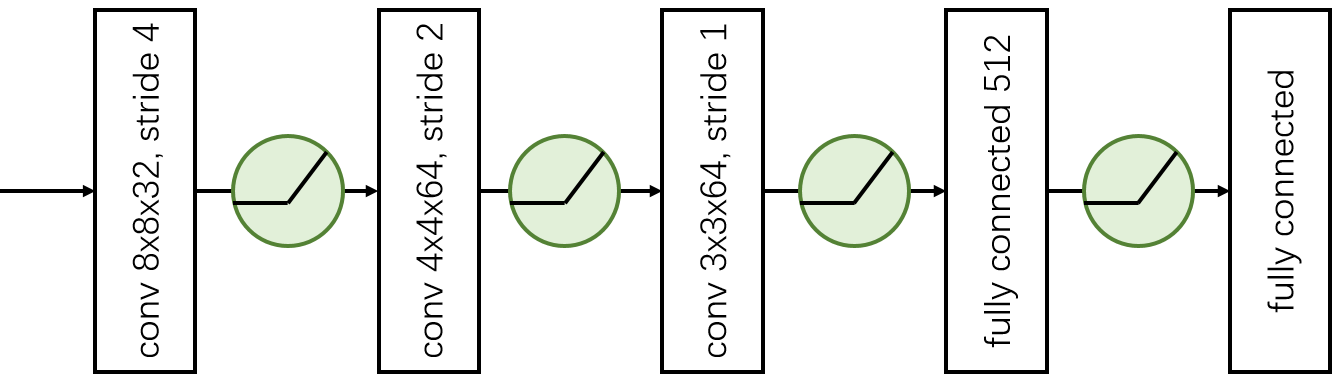
\includegraphics[width=1.0\linewidth]{net.png}
\end{center}
\caption{Structure of the CNN used for Q function}
\label{fig:net}
\end{figure}

Network structure is fixed for different games except for the last layer because the size of action set varies. The network receives $84\times 84$ 4 channel images as input, where the 4 channels are consecutive 4 frames. The network structure is shown in Figure~\ref{fig:net}. 

The $Y$ channel of every frame of the game is extracted to train the network. The reward at each time step is clipped to 1 or -1 or 0 to normalize the error for different games. Thus the learning rate is kept same. The agent works in an $\epsilon$-greedy way where the $\epsilon$ anneals linearly from 1 to 0.1 in the first million frames and fixed at 0.1 then. 50 million frames are used for training the network. The memory size is set to a million.

\subsection{Result}

\begin{figure*}
\begin{center}
   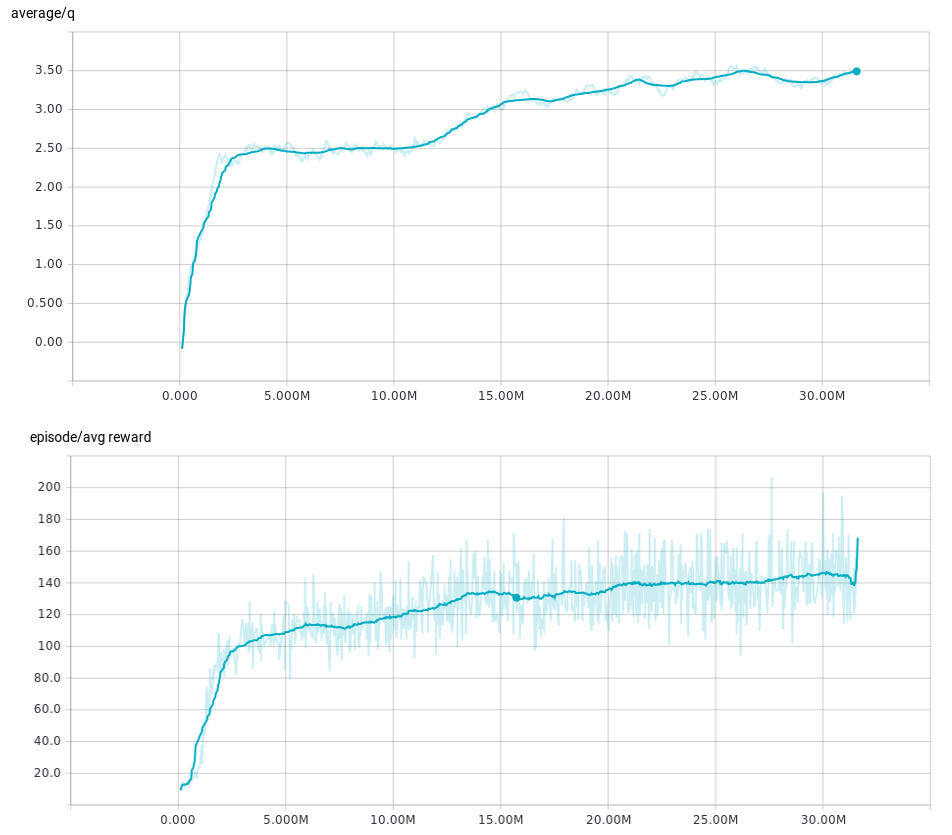
\includegraphics[width=0.65\linewidth]{space_res.PNG}
\end{center}
\caption{Space Invaders training log of the average q value and the average clipped reward gain in each episode.}
\label{fig:space_log}
\end{figure*}

The experiments we do are with 2 games, Breakout and Space Invaders. Limited by the computation resource available, the training process of Breakout is in $96\%$ process and that of Space Invaders is in $63\%$ process. Figure~\ref{fig:breakout_log} and Figure~\ref{fig:space_log} shows the log of the training process. 

\begin{figure*}
\begin{center}
   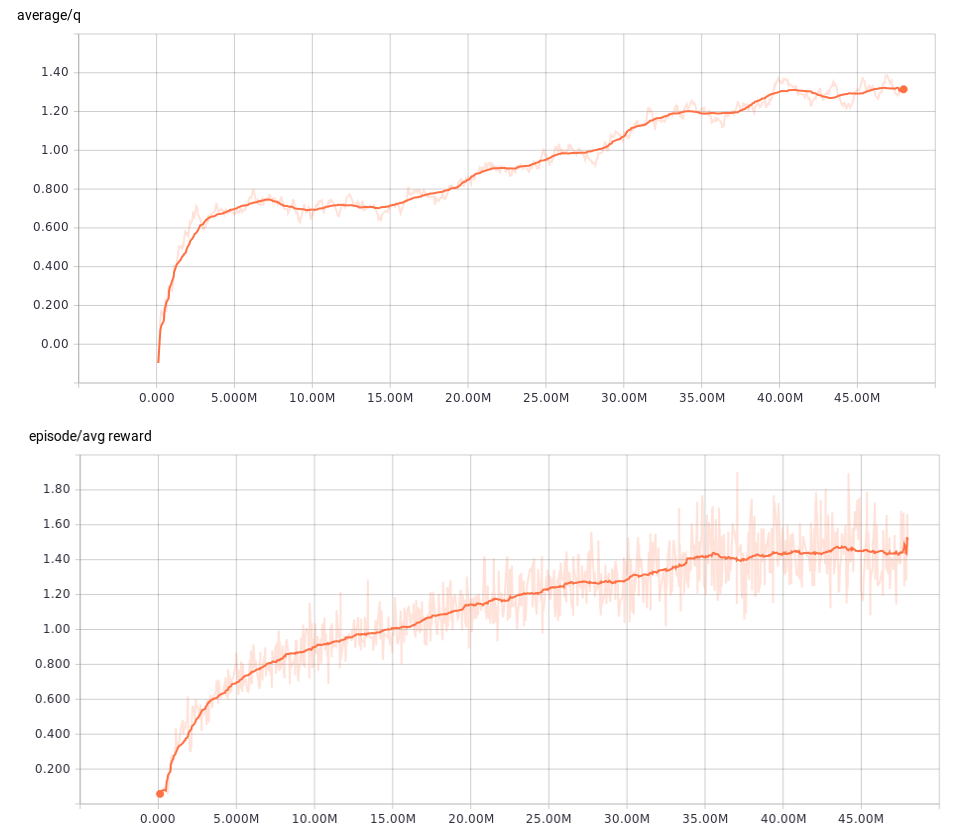
\includegraphics[width=0.65\linewidth]{breakout_res.PNG}
\end{center}
\caption{Breakout training log of the average q value and the average clipped reward gain in each episode.}
\label{fig:breakout_log}
\end{figure*}

\begin{figure}
\begin{center}
   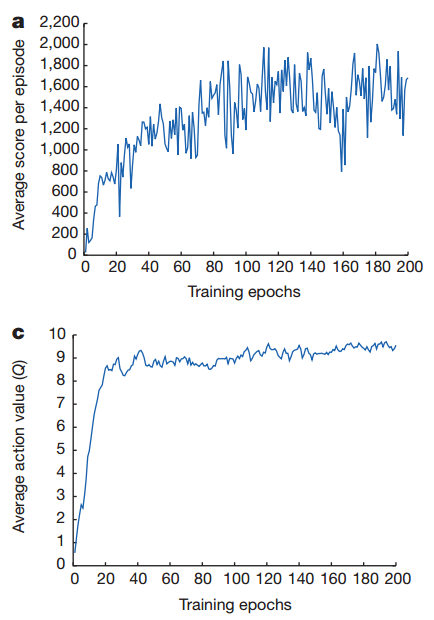
\includegraphics[width=1.0\linewidth]{paper_res.PNG}
\end{center}
\caption{Space Invaders training log of the the average score and the average action value in each episode.\cite{mnih2015human}}
\label{fig:paper_log}
\end{figure}

It is clear from the result that for both of the games, the average $q$ value, which is the estimated best value at each time step is increasing and the average reward in each episode is raising during the episode. This shows the validity of training. Figure~\ref{fig:paper_log} is from the paper which shows the training result on game Space Invader. There is still difference between our result and that reported in the paper. Further work should be done after training to checkout the details.

But even with the proposed training process in the paper, the performance of the agent is still showing great fluctuation. Moreover, the fluctuation is increasing during the training process. This may be a topic in future research.

\section{Discussion}

While the methods and tricks described in the paper achieved a huge success, there are still some spaces for improvement. There are two simple but effective methods that can be apply to Deep Q-Network for further performance improvement. 

First is Double Q-learning~\cite{van2015deep}. Original Deep Q-Network often tend to overestimate Q values of some actions through observations, which give agent a hard time to learn the best policy. The idea behind Double Q-learning is that change the way we estimate target Q value, from original  
\[
    target Q = r+\gamma \max\limits_{a^\prime} Q(s^\prime, a^\prime)
\]
to
\[
    target Q = r+\gamma Q(s^\prime, \argmax Q(s^\prime, a) )
\].
As we can see, instead of taking the max over Q values, it use Q network to chose an action, and target Q network to generate the target Q value for that action. By decoupling the action choice from the target Q value generation, it reduces the observed overestimation, and leads to much better performance in some situations.

Then is Dueling DQN~\cite{wang2015dueling}. The idea behind Dueling is quite simple: to give Q value a more fine degree definition. That is turn Q value to the sum of reward of state V(s) and reward of action A(s).
\[
    Q(s,a) = V(s) + A(s)
\]
Tune their parameters separately at the final layer and combine them to Q value finally. Decouple V(s) and A(s) actually give the agent ability to think of state and action separately, which makes more sense at some situations, hence leads to more robust estimation of policy and better performance. 

There are still more design spaces of DQN that can be explored, such as the combination with policy network and so on. RL is an interesting area and deserve our efforts to solve it. 

%-------------------------------------------------------------------------
{\small
\bibliographystyle{ieee}
\bibliography{egbib}
}

\end{CJK}
\end{document}
